\documentclass[11pt]{article} 
\usepackage[lmargin=1in,rmargin=1.75in,bmargin=1in,tmargin=.5in]{geometry}  
\usepackage{mdframed}
\usepackage{fontawesome5}

\input{hw-preamble}

\begin{document}
	
\hw{5}{October 9}
		
\problem (points removed for not answering!) Write down all outside resources you consulted, and the names of any other students that you worked with in any way. By turning in this homework, you acknowledge that you have read and abide by all course policies on outside resources and collaboration as stated in the course syllabus. If you did not work with others or use outside resources, then write that down.\\

\problem (15 points)
A company must assign workers to shifts. There are $n$ workers and $m$ shifts. 
Each worker $i\in[n]$ can work a subset $S_i\subseteq[m]$ of shifts, and each shift $j\in[m]$ requires exactly one worker. 
Your task is to design an algorithm that can  determine whether it is possible to assign every shift a distinct worker who can do it. 

\babc
\item (5 points)
Describe how to model this problem as a specific type of graph. 
Clearly define the two sets of vertices and the edges.

\item (6 points)
Construct a flow network based on your graph. 
Specify all vertices, edges, and capacities.

\item (4 points)
Explain how to use a maximum flow algorithm to determine whether all shifts can be assigned, and what condition on the flow value you check.
\eabc

\vfill

\problem (15 points total)
Aggieland is being evacuated due to a zombie outbreak! 
Our road network is modeled as a directed graph $G = (V, E)$, where each edge $(u, v)$ has a \emph{capacity} $c(u,v)$ representing the maximum number of students who can safely travel along that road before it becomes blocked (non-students are sacrificed to the zombies).

There are multiple \emph{evacuation centers} $S = \{ s_1, s_2, \dots, s_k \}$ where students start, and multiple \emph{safe zones} $T = \{ t_1, t_2, \dots, t_\ell \}$ where students can be evacuated to.
Each student must travel along a directed path from some $s_i \in S$ to some $t_j \in T$, and the total number of students using any edge cannot exceed its capacity.

\begin{center}
\faExclamationTriangle\faExclamationTriangle\faExclamationTriangle\faExclamationTriangle\faExclamationTriangle\faExclamationTriangle\faExclamationTriangle\faExclamationTriangle\faExclamationTriangle\faExclamationTriangle\faExclamationTriangle
\end{center}

You have access to a standard \emph{maximum flow algorithm} that works only for graphs with a single source and a single sink.
To use it, you decide to build an \emph{auxiliary graph} $G'$ and compute the maximum flow on $G'$.

\babc
\item (6 points)
Describe precisely how to construct the auxiliary graph $G'$ (its vertices, edges, and capacities) so that the maximum flow in $G'$ equals the \emph{maximum total number of students} that can be evacuated from all centers to all safe zones in $G$.

\item (5 points)
Explain why your construction correctly models the constraint that students can start from any evacuation center and end at any safe zone.

\item (4 points)
Explain why the value of the maximum flow in your constructed graph equals the maximum number of students that can be evacuated.
\eabc

\vfill

\problem (20 points)
Let $G = (L,R,E)$ be a bipartite graph. 
For a subset $A \subseteq L$, define the neighbors of $A$ formally by
\[N(A) = \{ v \in R : \exists\, u \in A \text{ such that } (u,v) \in E \}.\]

\babc
\item (4 points) Construct a flow network $G' = (V',E')$ as follows:
\begin{itemize}
\item 
Add a source $s$ and sink $t$.
\item 
Add edges $s \to u$ for all $u \in L$ with capacity $1$.
\item 
Add edges $v \to t$ for all $v \in R$ with capacity $1$.
\item 
For each $(u,v) \in E$, add edge $u \to v$ with capacity $1$.
\end{itemize}
Explain why any integral $s$-$t$ flow of value $k$ corresponds to a matching of size $k$ in $G$.

\item (4 points) 
State the Max-Flow Min-Cut Theorem. 
Then explain why $G$ has a matching saturating all vertices in $L$ if and only if the maximum flow in $G'$ has value $|L|$.

\item (6 points) 
Let $(S,T)$ be any $s$-$t$ cut in $G'$ with $s \in S$ and $t \in T$. 
Define
\[A = S \cap L, \quad B = S \cap R.\]
Show that the value of this cut is at least
\[|L \setminus A| + |N(A)|.\]
(HINT: Consider edges of the form $s \to u$, $u \to v$, and $v \to t$ separately.)

\item (6 points) 
Using the previous parts, prove that $G$ has a matching saturating all vertices in $L$ if and only if
\[|N(A)| \ge |A| \quad \text{for all } A \subseteq L.\]
(This is known as Hall�s Marriage Theorem.)
\eabc

\newpage
\hrule
\vspace{0.5in}
\begin{center}
PRACTICE PROBLEMS -- DO NOT TURN IN
\end{center}
\vspace{0.5in}
\noindent

\exercise
Consider the following flow on a network graph.  
  \begin{figure}[!htb]
\centering
  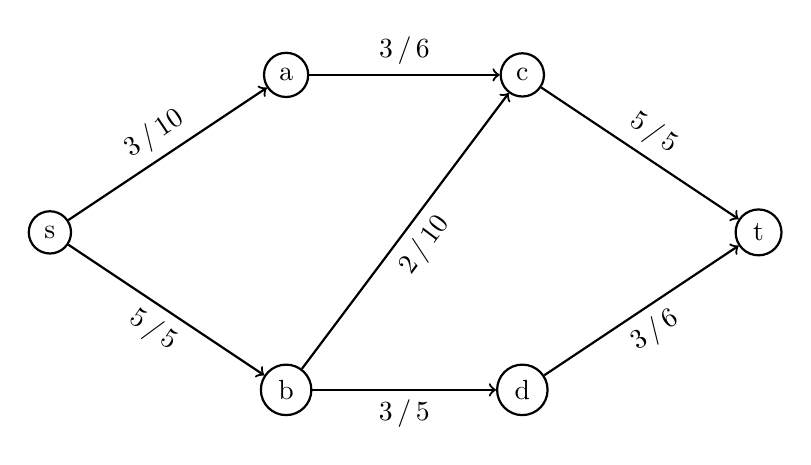
\begin{tikzpicture}[node distance=2cm, auto, thick, every node/.style={sloped,allow upside down}]

    % Node definitions
    \node (s) at (0, 0) [circle, draw] {s};
    \node (a) at (3, 2) [circle, draw] {a};
    \node (b) at (3, -2) [circle, draw] {b};
    \node (c) at (6, 2) [circle, draw] {c};
    \node (d) at (6, -2) [circle, draw] {d};
    \node (t) at (9, 0) [circle, draw] {t};

    % Edge definitions with flow over capacity
    \draw[->, thick] (s) -- (a) node[midway, above] {3\,/\,10};
    \draw[->, thick] (s) -- (b) node[midway, below] {5\,/\,5};
    \draw[->, thick] (a) -- (c) node[midway, above] {3\,/\,6};
    \draw[->, thick] (b) -- (d) node[midway, below] {3\,/\,5};
    \draw[->, thick] (c) -- (t) node[midway, above] {5\,/\,5};
    \draw[->, thick] (d) -- (t) node[midway, below] {3\,/\,6};
    %\draw[->, thick] (a) -- (d) node[pos=0.25, below] {0\,/\,7};
    \draw[->, thick] (b) -- (c) node[pos=0.5, below] {2\,/\,10};
\end{tikzpicture}
\caption{Figure for Long Answer Question \#3}
\label{fig:2}
\end{figure}

	\begin{enumerate}[(a)]
		\item (9 points) For the flow network graph in Figure~\ref{fig:2}, do all of the following:
  \begin{enumerate}[(i)]
      \item \textbf{CLEARLY} draw the residual graph
      \item Write down the edges in an augmenting path
      \item Draw a maximum $s-t$ flow \textbf{AND} compute the value of the flow
  \end{enumerate}
\vfill
  \begin{figure}[!htb]
\centering
  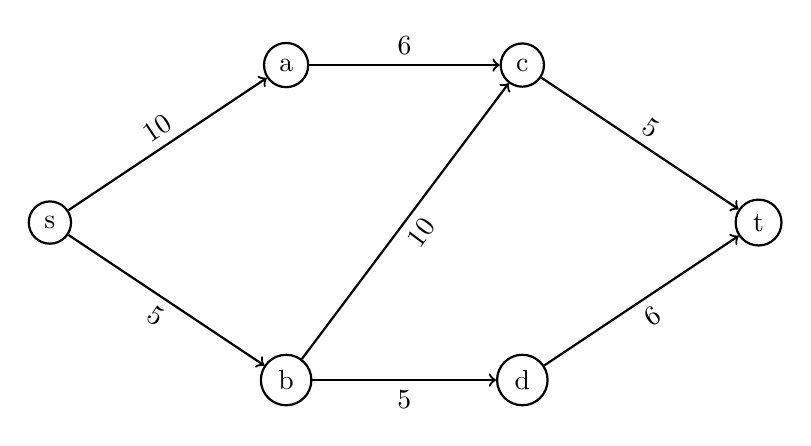
\begin{tikzpicture}[node distance=2cm, auto, thick, every node/.style={sloped,allow upside down}]

    % Node definitions
    \node (s) at (0, 0) [circle, draw] {s};
    \node (a) at (3, 2) [circle, draw] {a};
    \node (b) at (3, -2) [circle, draw] {b};
    \node (c) at (6, 2) [circle, draw] {c};
    \node (d) at (6, -2) [circle, draw] {d};
    \node (t) at (9, 0) [circle, draw] {t};

    % Edge definitions with flow over capacity
    \draw[->, thick] (s) -- (a) node[midway, above] {10};
    \draw[->, thick] (s) -- (b) node[midway, below] {5};
    \draw[->, thick] (a) -- (c) node[midway, above] {6};
    \draw[->, thick] (b) -- (d) node[midway, below] {5};
    \draw[->, thick] (c) -- (t) node[midway, above] {5};
    \draw[->, thick] (d) -- (t) node[midway, below] {6};
    %\draw[->, thick] (a) -- (d) node[pos=0.25, below] {0\,/\,7};
    \draw[->, thick] (b) -- (c) node[pos=0.5, below] {10};
\end{tikzpicture}
\caption{Figure for Long Answer Question \#3}
\label{fig:3}
\end{figure}
\item (6 points) For the same network graph in Figure~\ref{fig:3}, do all of the following:
\begin{enumerate}[(i)]
\item 
Find a minimum $s-t$ cut \textbf{AND} compute the value of the cut. 
\item 
Using your answer to part 3a(iii), prove the optimality of the minimum $s-t$ cut that you found. 
\end{enumerate}
  \vfill
	\end{enumerate}
		\vfill

\exercise
Consider the following flow network with source $s$ and sink $t$:

\begin{center}
\begin{tabular}{c}
Edges (capacity, flow): \\
$s \to a$ (10, 6), \quad $s \to b$ (5, 5) \\
$a \to b$ (15, 3), \quad $a \to t$ (10, 6) \\
$b \to t$ (10, 8)
\end{tabular}
\end{center}

\babc
\item 
Compute the residual capacity of every forward and backward edge.
\item 
List all edges in the residual graph $G_f$.
\item 
Is there an augmenting path from $s$ to $t$, i.e., an $s$-$t$ path in $G_f$? If so, give one.
\item 
Compute the bottleneck capacity of this path.
\item 
Update the flow values along the path.
\item 
What is the new value of the flow?
\eabc
\vfill

\exercise
\babc
\item 
Explain why the absence of an $s$-$t$ path in the residual graph implies that no additional flow can be sent.
\item 
Using the idea of cuts, argue why the current flow must be maximum.
\eabc
\vfill

\exercise
Suppose you want to find the maximum flow on a network graph that has sources $s_1, s_2$ and one sink $t$.
\babc
\item 
Describe how to construct a new graph with a single source $s$.
\item 
What capacities should you assign to the new edges?
\item 
Explain why this transformation preserves the maximum flow.
\eabc
\vfill

\newpage
\challenge
In a directed graph $G = (V,E)$, suppose each vertex $v \in V$ has an associated integer \emph{demand} $d(v)$, where:
\begin{itemize}
\item 
$d(v) > 0$ means $v$ requires $d(v)$ units of incoming flow,
\item 
$d(v) < 0$ means $v$ supplies $-d(v)$ units of flow,
\item 
$d(v) = 0$ means $v$ has no net demand.
\end{itemize}
Each edge $(u,v)$ has capacity $c(u,v)$. 
A flow $f$ is said to be \emph{feasible} if:
\begin{itemize}
\item 
$0 \le f(u,v) \le c(u,v)$ for all edges,
\item 
for every vertex $v \in V$,
\[\sum_{u:(u,v)\in E} f(u,v) - \sum_{w:(v,w)\in E} f(v,w) = d(v).\]
\end{itemize}
In other words, the net incoming flow at each vertex must equal its demand.

\babc
\item 
Explain why a necessary condition for a feasible flow to exist is
\[\sum_{v \in V} d(v) = 0.\]
\item 
Describe how to construct a new graph $G'$ with a single source $s$ and sink $t$ such that a feasible flow in $G$ exists if and only if a maximum flow in $G'$ saturates all edges out of $s$.

(You should specify all vertices, edges, and capacities in your construction.)

\item 
Explain why your construction is correct. 
In particular, argue how satisfying all demands corresponds to saturating the edges from $s$.

\item 
What is the runtime of your algorithm in terms of $|V|$ and $|E|$?
\eabc

\end{document}